% !TEX TS-program = pdflatex
% !TEX encoding = UTF-8 Unicode

% This is a simple template for a LaTeX document using the "article" class.
% See "book", "report", "letter" for other types of document.

\documentclass[11pt]{article} % use larger type; default would be 10pt

\usepackage[utf8]{inputenc} % set input encoding (not needed with XeLaTeX)

%%% Examples of Article customizations
% These packages are optional, depending whether you want the features they provide.
% See the LaTeX Companion or other references for full information.

%%% PAGE DIMENSIONS
\usepackage{geometry} % to change the page dimensions
\geometry{a4paper} % or letterpaper (US) or a5paper or....
% \geometry{margin=2in} % for example, change the margins to 2 inches all round
% \geometry{landscape} % set up the page for landscape
%   read geometry.pdf for detailed page layout information

\usepackage{graphicx} % support the \includegraphics command and options

% \usepackage[parfill]{parskip} % Activate to begin paragraphs with an empty line rather than an indent

%%% PACKAGES
\usepackage{booktabs} % for much better looking tables
\usepackage{array} % for better arrays (eg matrices) in maths
\usepackage{paralist} % very flexible & customisable lists (eg. enumerate/itemize, etc.)
\usepackage{verbatim} % adds environment for commenting out blocks of text & for better verbatim
\usepackage{subfig} % make it possible to include more than one captioned figure/table in a single float
% These packages are all incorporated in the memoir class to one degree or another...

%%% HEADERS & FOOTERS
\usepackage{fancyhdr} % This should be set AFTER setting up the page geometry
\pagestyle{fancy} % options: empty , plain , fancy
\renewcommand{\headrulewidth}{0pt} % customise the layout...
\lhead{}\chead{}\rhead{}
\lfoot{}\cfoot{\thepage}\rfoot{}

%%% SECTION TITLE APPEARANCE
\usepackage{sectsty}
\allsectionsfont{\sffamily\mdseries\upshape} % (See the fntguide.pdf for font help)
% (This matches ConTeXt defaults)

%%% ToC (table of contents) APPEARANCE
\usepackage[nottoc,notlof,notlot]{tocbibind} % Put the bibliography in the ToC
\usepackage[titles,subfigure]{tocloft} % Alter the style of the Table of Contents
\usepackage{graphicx}
\renewcommand{\cftsecfont}{\rmfamily\mdseries\upshape}
\renewcommand{\cftsecpagefont}{\rmfamily\mdseries\upshape} % No bold!

%%% END Article customizations

%%% The "real" document content comes below...

\title{Writeup For the final project}
\author{Ali Lotfi}
%\date{} % Activate to display a given date or no date (if empty),
         % otherwise the current date is printed 

\begin{document}
\maketitle

\section{Tests we ran}
I ran 8 sets, each 500 tests for minheap implemented and also STL and linked list priority queue.
The results are set to pop as we run the code and also I have included 6 different graphs for each method as far as average time and standard deviation.
The min heap which we implemented work faster than STL and the conjecture that all of them are correlated to the size of the data was accurate.
for implementing LL we have the following elements in the class:\\
push()\\
pop()\\
deletelist()\\
printlist()\\
For minheap we implemented:\\
push()\\
pop()\\
printheap()\\
heap[]\\
currentsize\\
minheapify(int)\\
And also for STL I didnt have to do much other than following the lecture.
For almost all of them I had to make a structure patient with elements name, priority and treatment. There is also an extra function called helper function which does lexiographic ordering on patients since priority is more important.
The time complexity of removing $O(logn)$ could not be seen in the graphs since it is part of what we measured as far as time. 
\begin{figure}[ht!]
\centering
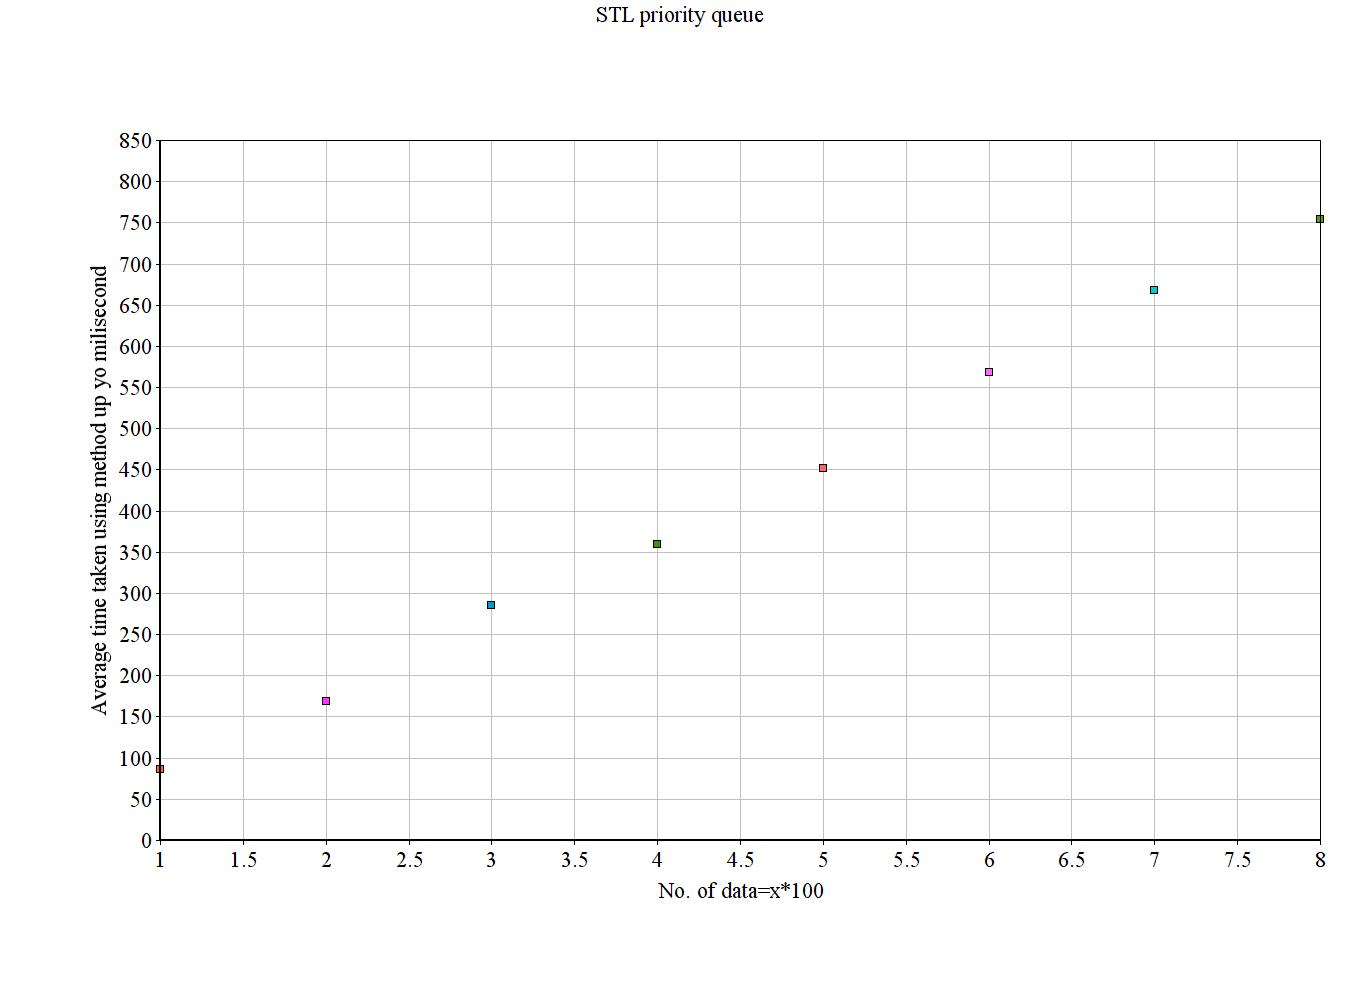
\includegraphics[width=120mm]{1.jpg}

\end{figure}
\begin{figure}[ht!]
\centering
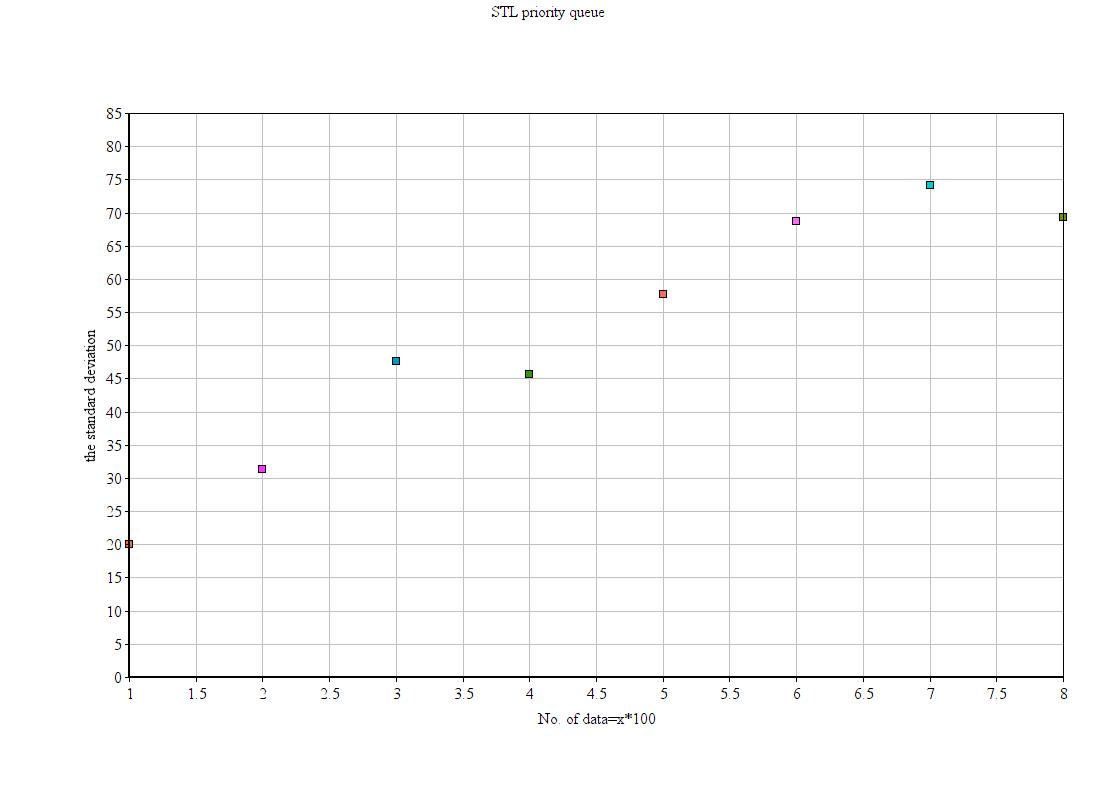
\includegraphics[width=120mm]{2.jpg}

\end{figure}
\begin{figure}[ht!]
\centering
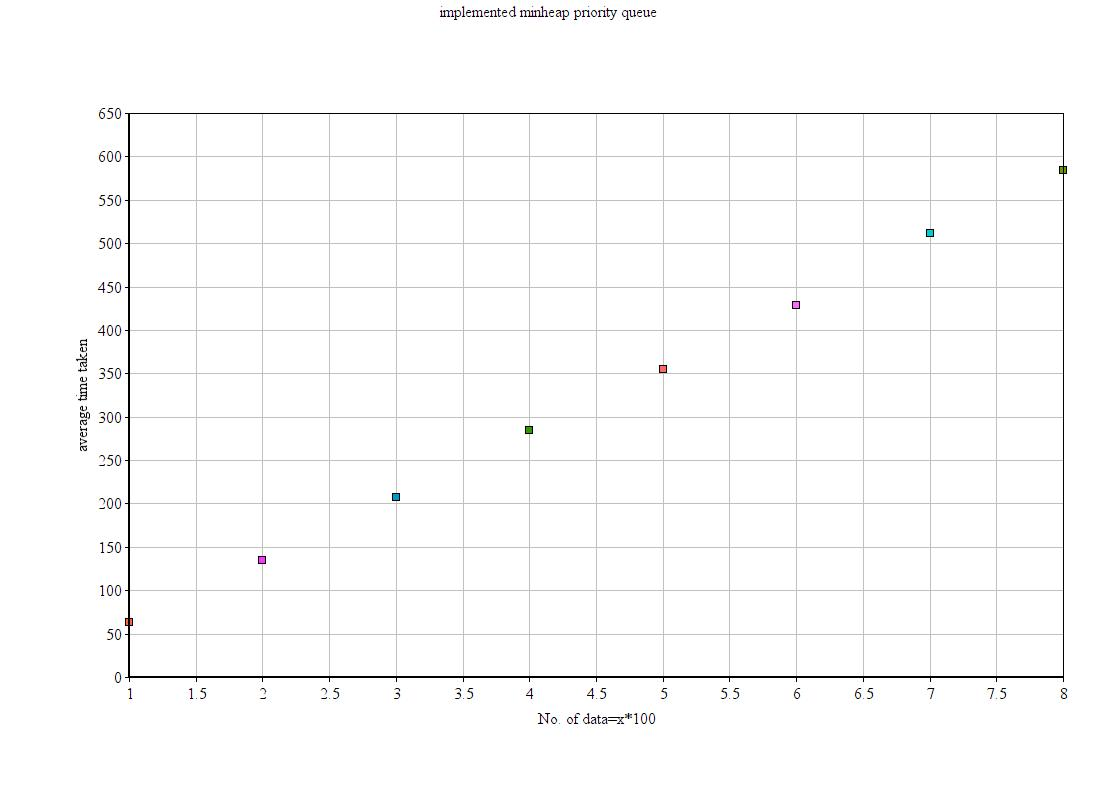
\includegraphics[width=120mm]{3.jpg}

\end{figure}
\begin{figure}[ht!]
\centering
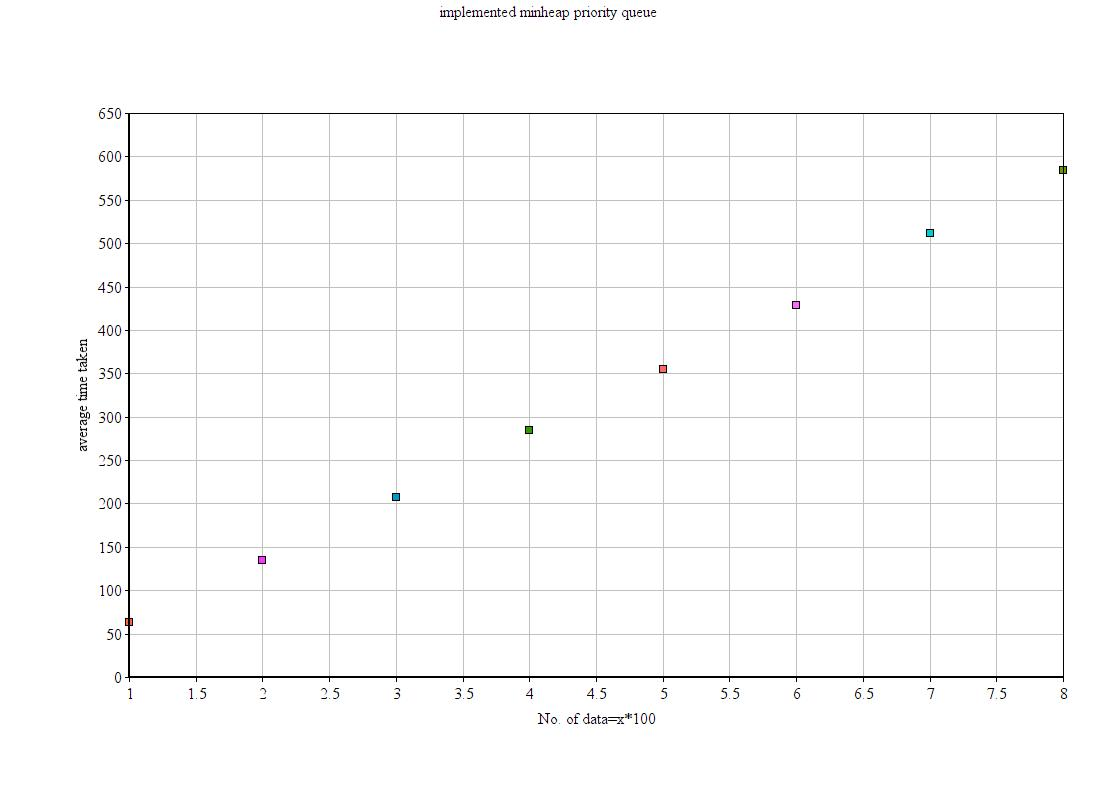
\includegraphics[width=120mm]{4.jpg}

\end{figure}
\begin{figure}[ht!]
\centering
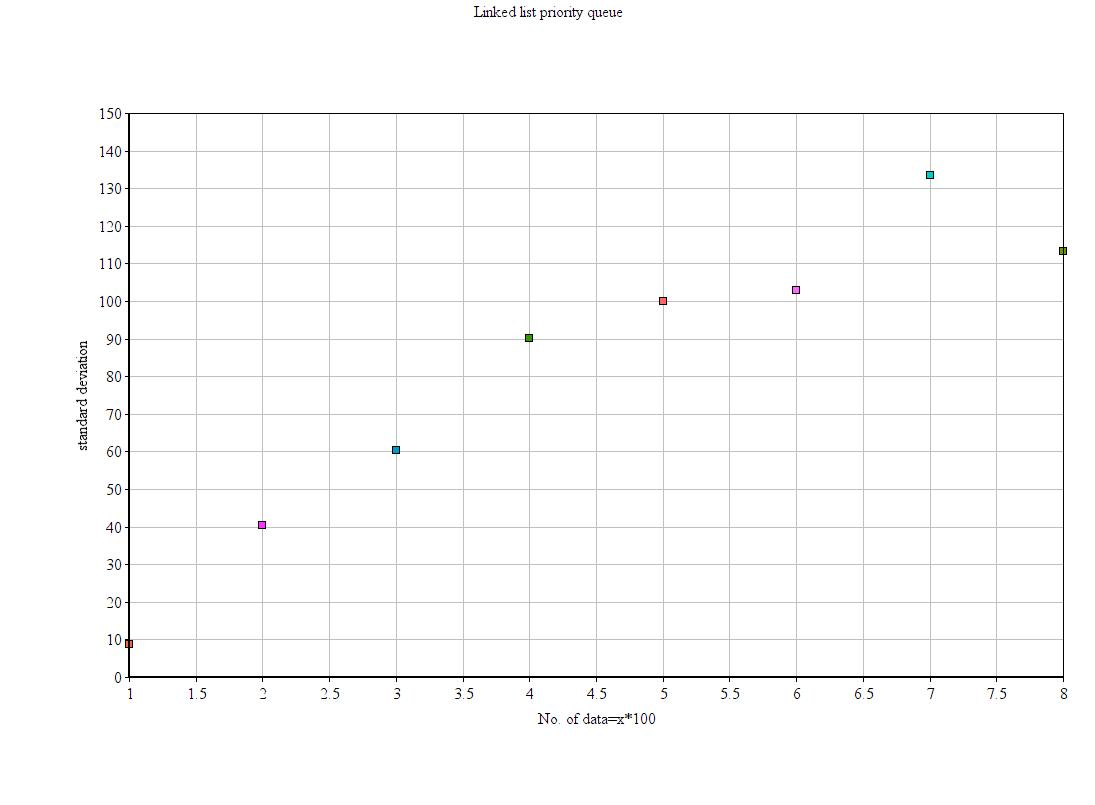
\includegraphics[width=120mm]{5.jpg}

\end{figure}
\begin{figure}[ht!]
\centering
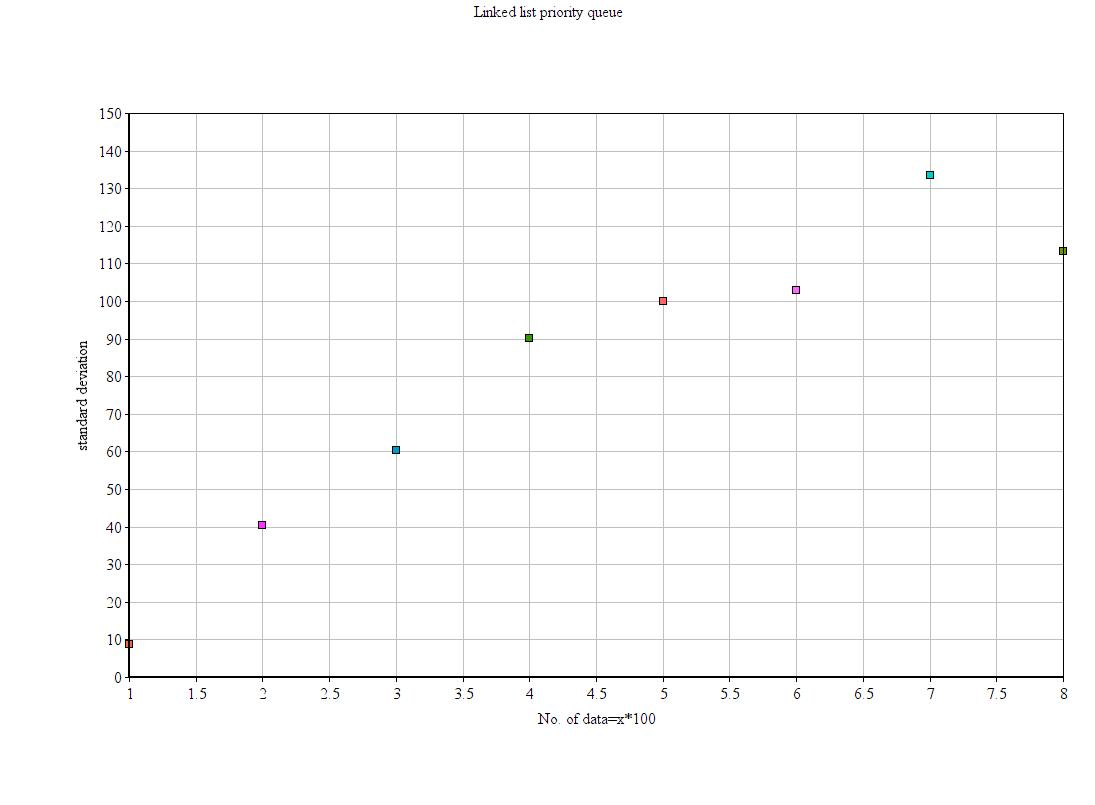
\includegraphics[width=120mm]{6.jpg}

\end{figure}
\end{document}
